\documentclass[10pt, conference]{IEEEtran}

\newcommand{\ignore}[1]{}

% *** MISC UTILITY PACKAGES ***
%
%\usepackage{ifpdf}
% Heiko Oberdiek's ifpdf.sty is very useful if you need conditional
% compilation based on whether the output is pdf or dvi.
% usage:
% \ifpdf
%   % pdf code
% \else
%   % dvi code
% \fi
% The latest version of ifpdf.sty can be obtained from:
% http://www.ctan.org/tex-archive/macros/latex/contrib/oberdiek/
% Also, note that IEEEtran.cls V1.7 and later provides a builtin
% \ifCLASSINFOpdf conditional that works the same way.
% When switching from latex to pdflatex and vice-versa, the compiler may
% have to be run twice to clear warning/error messages.






% *** CITATION PACKAGES ***
%
%\usepackage{cite}
% cite.sty was written by Donald Arseneau
% V1.6 and later of IEEEtran pre-defines the format of the cite.sty package
% \cite{} output to follow that of IEEE. Loading the cite package will
% result in citation numbers being automatically sorted and properly
% "compressed/ranged". e.g., [1], [9], [2], [7], [5], [6] without using
% cite.sty will become [1], [2], [5]--[7], [9] using cite.sty. cite.sty's
% \cite will automatically add leading space, if needed. Use cite.sty's
% noadjust option (cite.sty V3.8 and later) if you want to turn this off.
% cite.sty is already installed on most LaTeX systems. Be sure and use
% version 4.0 (2003-05-27) and later if using hyperref.sty. cite.sty does
% not currently provide for hyperlinked citations.
% The latest version can be obtained at:
% http://www.ctan.org/tex-archive/macros/latex/contrib/cite/
% The documentation is contained in the cite.sty file itself.







% *** GRAPHICS RELATED PACKAGES ***
\usepackage[pdftex]{graphicx}
\usepackage{xcolor}
\usepackage{caption} %needed to make captions on figure* centered
\graphicspath{{./figures/}}
\DeclareGraphicsExtensions{.pdf,.png}
\usepackage[draft]{hyperref}



% *** MATH PACKAGES ***
%
%\usepackage[cmex10]{amsmath}
% A popular package from the American Mathematical Society that provides
% many useful and powerful commands for dealing with mathematics. If using
% it, be sure to load this package with the cmex10 option to ensure that
% only type 1 fonts will utilized at all point sizes. Without this option,
% it is possible that some math symbols, particularly those within
% footnotes, will be rendered in bitmap form which will result in a
% document that can not be IEEE Xplore compliant!
%
% Also, note that the amsmath package sets \interdisplaylinepenalty to 10000
% thus preventing page breaks from occurring within multiline equations. Use:
%\interdisplaylinepenalty=2500
% after loading amsmath to restore such page breaks as IEEEtran.cls normally
% does. amsmath.sty is already installed on most LaTeX systems. The latest
% version and documentation can be obtained at:
% http://www.ctan.org/tex-archive/macros/latex/required/amslatex/math/





% *** SPECIALIZED LIST PACKAGES ***
%
%\usepackage{algorithmic}
% algorithmic.sty was written by Peter Williams and Rogerio Brito.
% This package provides an algorithmic environment fo describing algorithms.
% You can use the algorithmic environment in-text or within a figure
% environment to provide for a floating algorithm. Do NOT use the algorithm
% floating environment provided by algorithm.sty (by the same authors) or
% algorithm2e.sty (by Christophe Fiorio) as IEEE does not use dedicated
% algorithm float types and packages that provide these will not provide
% correct IEEE style captions. The latest version and documentation of
% algorithmic.sty can be obtained at:
% http://www.ctan.org/tex-archive/macros/latex/contrib/algorithms/
% There is also a support site at:
% http://algorithms.berlios.de/index.html
% Also of interest may be the (relatively newer and more customizable)
% algorithmicx.sty package by Szasz Janos:
% http://www.ctan.org/tex-archive/macros/latex/contrib/algorithmicx/




% *** ALIGNMENT PACKAGES ***
%
%\usepackage{array}
% Frank Mittelbach's and David Carlisle's array.sty patches and improves
% the standard LaTeX2e array and tabular environments to provide better
% appearance and additional user controls. As the default LaTeX2e table
% generation code is lacking to the point of almost being broken with
% respect to the quality of the end results, all users are strongly
% advised to use an enhanced (at the very least that provided by array.sty)
% set of table tools. array.sty is already installed on most systems. The
% latest version and documentation can be obtained at:
% http://www.ctan.org/tex-archive/macros/latex/required/tools/


%\usepackage{mdwmath}
%\usepackage{mdwtab}
% Also highly recommended is Mark Wooding's extremely powerful MDW tools,
% especially mdwmath.sty and mdwtab.sty which are used to format equations
% and tables, respectively. The MDWtools set is already installed on most
% LaTeX systems. The lastest version and documentation is available at:
% http://www.ctan.org/tex-archive/macros/latex/contrib/mdwtools/


% IEEEtran contains the IEEEeqnarray family of commands that can be used to
% generate multiline equations as well as matrices, tables, etc., of high
% quality.


%\usepackage{eqparbox}
% Also of notable interest is Scott Pakin's eqparbox package for creating
% (automatically sized) equal width boxes - aka "natural width parboxes".
% Available at:
% http://www.ctan.org/tex-archive/macros/latex/contrib/eqparbox/





% *** SUBFIGURE PACKAGES ***
%\usepackage[tight,footnotesize]{subfigure}
% subfigure.sty was written by Steven Douglas Cochran. This package makes it
% easy to put subfigures in your figures. e.g., "Figure 1a and 1b". For IEEE
% work, it is a good idea to load it with the tight package option to reduce
% the amount of white space around the subfigures. subfigure.sty is already
% installed on most LaTeX systems. The latest version and documentation can
% be obtained at:
% http://www.ctan.org/tex-archive/obsolete/macros/latex/contrib/subfigure/
% subfigure.sty has been superceeded by subfig.sty.



%\usepackage[caption=false]{caption}
%\usepackage[font=footnotesize]{subfig}
% subfig.sty, also written by Steven Douglas Cochran, is the modern
% replacement for subfigure.sty. However, subfig.sty requires and
% automatically loads Axel Sommerfeldt's caption.sty which will override
% IEEEtran.cls handling of captions and this will result in nonIEEE style
% figure/table captions. To prevent this problem, be sure and preload
% caption.sty with its "caption=false" package option. This is will preserve
% IEEEtran.cls handing of captions. Version 1.3 (2005/06/28) and later 
% (recommended due to many improvements over 1.2) of subfig.sty supports
% the caption=false option directly:
%\usepackage[caption=false,font=footnotesize]{subfig}
%
% The latest version and documentation can be obtained at:
% http://www.ctan.org/tex-archive/macros/latex/contrib/subfig/
% The latest version and documentation of caption.sty can be obtained at:
% http://www.ctan.org/tex-archive/macros/latex/contrib/caption/




% *** FLOAT PACKAGES ***
%
%\usepackage{fixltx2e}
% fixltx2e, the successor to the earlier fix2col.sty, was written by
% Frank Mittelbach and David Carlisle. This package corrects a few problems
% in the LaTeX2e kernel, the most notable of which is that in current
% LaTeX2e releases, the ordering of single and double column floats is not
% guaranteed to be preserved. Thus, an unpatched LaTeX2e can allow a
% single column figure to be placed prior to an earlier double column
% figure. The latest version and documentation can be found at:
% http://www.ctan.org/tex-archive/macros/latex/base/



%\usepackage{stfloats}
% stfloats.sty was written by Sigitas Tolusis. This package gives LaTeX2e
% the ability to do double column floats at the bottom of the page as well
% as the top. (e.g., "\begin{figure*}[!b]" is not normally possible in
% LaTeX2e). It also provides a command:
%\fnbelowfloat
% to enable the placement of footnotes below bottom floats (the standard
% LaTeX2e kernel puts them above bottom floats). This is an invasive package
% which rewrites many portions of the LaTeX2e float routines. It may not work
% with other packages that modify the LaTeX2e float routines. The latest
% version and documentation can be obtained at:
% http://www.ctan.org/tex-archive/macros/latex/contrib/sttools/
% Documentation is contained in the stfloats.sty comments as well as in the
% presfull.pdf file. Do not use the stfloats baselinefloat ability as IEEE
% does not allow \baselineskip to stretch. Authors submitting work to the
% IEEE should note that IEEE rarely uses double column equations and
% that authors should try to avoid such use. Do not be tempted to use the
% cuted.sty or midfloat.sty packages (also by Sigitas Tolusis) as IEEE does
% not format its papers in such ways.





% *** PDF, URL AND HYPERLINK PACKAGES ***
%
%\usepackage{url}
% url.sty was written by Donald Arseneau. It provides better support for
% handling and breaking URLs. url.sty is already installed on most LaTeX
% systems. The latest version can be obtained at:
% http://www.ctan.org/tex-archive/macros/latex/contrib/misc/
% Read the url.sty source comments for usage information. Basically,
% \url{my_url_here}.





% *** Do not adjust lengths that control margins, column widths, etc. ***
% *** Do not use packages that alter fonts (such as pslatex).         ***
% There should be no need to do such things with IEEEtran.cls V1.6 and later.
% (Unless specifically asked to do so by the journal or conference you plan
% to submit to, of course. )


% correct bad hyphenation here
\hyphenation{Dev-Ops}


\begin{document}
%
% paper title
% can use linebreaks \\ within to get better formatting as desired
\title{Seneca: Model Optimization as a service by Serverless}


% author names and affiliations
% use a multiple column layout for up to two different
% affiliations

\author{\IEEEauthorblockN{Michael Zhang, Chandra Krintz, Rich Wolski}
\IEEEauthorblockA{Dept. of Computer Science \\
Univeristy of California, Santa Barbara\\
\{lebo, ckrintz, rich\}@cs.ucsb.edu}
}

% conference papers do not typically use \thanks and this command
% is locked out in conference mode. If really needed, such as for
% the acknowledgment of grants, issue a \IEEEoverridecommandlockouts
% after \documentclass

% for over three affiliations, or if they all won't fit within the width
% of the page, use this alternative format:
% 
%\author{\IEEEauthorblockN{Michael Shell\IEEEauthorrefmark{1},
%Homer Simpson\IEEEauthorrefmark{2},
%James Kirk\IEEEauthorrefmark{3}, 
%Montgomery Scott\IEEEauthorrefmark{3} and
%Eldon Tyrell\IEEEauthorrefmark{4}}
%\IEEEauthorblockA{\IEEEauthorrefmark{1}School of Electrical and Computer Engineering\\
%Georgia Institute of Technology,
%Atlanta, Georgia 30332--0250\\ Email: see http://www.michaelshell.org/contact.html}
%\IEEEauthorblockA{\IEEEauthorrefmark{2}Twentieth Century Fox, Springfield, USA\\
%Email: homer@thesimpsons.com}
%\IEEEauthorblockA{\IEEEauthorrefmark{3}Starfleet Academy, San Francisco, California 96678-2391\\
%Telephone: (800) 555--1212, Fax: (888) 555--1212}
%\IEEEauthorblockA{\IEEEauthorrefmark{4}Tyrell Inc., 123 Replicant Street, Los Angeles, California 90210--4321}}









% make the title area
\maketitle


\begin{abstract}
\label{sec:abstract}
The goal of our work is to simplify and expedite the 
construction and evaluation of machine learning models 
using autoscaled cloud computing systems and services.
To enable this, we develop an open source system, called Seneca, that leverages
the serverless programming model and its implementation in Amazon Web Services
(AWS) Lambda.  
Seneca takes a machine learning application, dataset, and a list of 
possible hyperparameter options.  It automatically constructs an AWS Lambda
handler that ingresses and splits the dataset into training
and testing subsets, and constructs, tests, and evaluates (i.e. scores) a machine
learning model for a given set of hyperparameter values.  Seneca concurrently invokes
functions for all combinations of the hyperparameters specified.
It then returns the configuration (or model) that results in the best score 
to the user.  

We present the design and implementation of Seneca and introduce an extension to the
system that automatically optimizes memory use by the functions.  
Our empirical evaluation using multiple predictive machine learning applications 
for regression and classification shows that Seneca is able to quickly
identify the best performing model for the programs and datasets that we consider.
Moreover, its memory optimization reduces the cost of using Seneca 
by 10-30\% for the applications studied.

%The involvement of manual operations and domain expertise makes traditional model optimization process expensive, time-consuming and not guaranteed the optimal solution. The emergence of serverless computing offers the potential to optimize models in an auto-scaling and micro-billing fashion. In this paper, we present Seneca -- a framework for machine learning model optimization on serverless computing platform. Its automated pipeline consists of packaging, deployment, serverless function optimization and hyperparameter tuning, which provides a cost-effective, high-performing and reliable model optimization service. We evaluate Seneca by performance, cost and latency analysis on multiple regression and classification applications. The result demonstrates Seneca streamlines model deployment and optimization in agile and economical fashion.

\end{abstract}

\begin{IEEEkeywords}
Serverless computing; Model optimization; Hyperparameters tuning
\end{IEEEkeywords}


% For peer review papers, you can put extra information on the cover
% page as needed:
% \ifCLASSOPTIONpeerreview
% \begin{center} \bfseries EDICS Category: 3-BBND \end{center}
% \fi
%
% For peerreview papers, this IEEEtran command inserts a page break and
% creates the second title. It will be ignored for other modes.
\IEEEpeerreviewmaketitle



\section{Introduction}
\label{sec:intro}
The scale and elasticity of cloud computing systems have 
fueled remarkable innovation and unprecedented commercial 
investment.  Cloud users ``rent'' virtualized resources (while sharing
the underlying physical resources) on a pay-per-use basis
in exchange for availability guarantees specified via service level
agreements (SLAs). Uniquely, cloud systems can be configured 
to add and remove resources and services,
automatically and on-demand, based on load 
or as required by executing applications.

To date however, cloud use has been limited to large-scale 
implementations of enterprise services, such as
object storage, databases, queuing systems, and web and application servers.
The reason for this is that it is very
challenging, even for expert users, to configure complex
distributed systems for application use, 
and to leverage the elasticity (auto-scaling) that
clouds offer. To address this challenge, cloud providers 
have started to offer cloud programming and execution environments
under the moniker of \textit{serverless} 
computing~\cite{xxx,yyy,zzz}.  Serverless
systems automatically configure, manage, and scale applications
to significantly simplify and broaden participation in (by less expert
users) the use of cloud systems.
%xxx: http://shivaram.org/publications/pywren-socc17.pdf
%yyy: http://cidrdb.org/cidr2019/papers/p119-hellerstein-cidr19.pdf
%zzz: L. Wang, M. Li, Y. Zhang, T. Ristenpart, and M. Swift. “Peek- ing Behind the Curtains of Serverless Platforms”. In: USENIX ATC. Boston, MA: USENIX Association, 2018

Using the serverless model, applications developers upload 
arbitrary computations in high level languages
as stateless functions to these cloud-hosted services, along with a
specification conditions under which each
function should be triggered.  Functions are invoked (triggered)
automatically by the cloud in response to updates to other cloud services
(e.g. storage, queues, notification services, among others). They
communicate, persist, and access data only 
via their inputs or shared, remote storage.  
As a result, serverless applications are inherently elastic and can 
implement highly concurrent and parallel tasks.
In public clouds, users pay a small fee for the resources their 
functions use during execution, resulting in very low cost cloud use.
Although now available from all public cloud providers and as open 
source for private cloud systems, 
AWS Lambda~\cite{awslambda} was the first and is now the 
most popular and most advanced serverless public cloud service 
available today.
%awslambda: https://docs.aws.amazon.com/lambda/latest/dg/lambda-dg.pdf

In this work, we investigate the efficacy of using AWS Lambda
for tuning machine learning applications.
To date, Lambda has not be heavily used for training and evaluating
machine learning models because of a concern that 
doing so will result in high overhead (i.e. be costly) because
of the stateless nature of serverless functions~\cite{ref:onesteptwostep}.
At the same time, identifying the ``best'' configuration for advanced
machine learning models is challenging given the large number of configuration
options, i.e., hyperparameters, typical of models today.
Hyperparameters governs the learning process of machine learning applications.
Given that parameter sweeps are embarrassingly parallel, we believe
that such tuning is a good fit for the serverless model.
To investigate this potential, its overhead, and to simplify the 
use of Lambda for training, testing, and evaluation machine learning models, 
we design and develop a new system and toolset called \textit{Seneca}.

Specifically, Seneca implements, packages, and deploys 
machine learning applications as stateless functions to AWS Lambda.
It then orchestrates exhaustive evaluation of hyperparameter settings
to identify the best performing model (for a given dataset) by
comparing the error and accuracy across models.  Users present
Seneca with their application, a range of values for 
each hyperparameter (or the default can be used), and a dataset.
Seneca produces, tests, and evaluates models for all combinations 
of hyperparameters and returns to the user, 
the set of parameters (or the model itself) that produces
the best cross-validation score (e.g. lowest squared error or highest
accuracy).

We deploy Seneca on AWS Lambda and evaluate its tuning performance, cost,
and memory use for six machine learning applications and datasets. We 
find that Seneca is effective for quickly training these
models and identifying the best performing hyperparameter setting for 
these applications. We also find 
Seneca to be very low cost and able to automatically 
identify the 
best memory configuration for each application further lowering its 
by 10-30\%.
We intend to make Seneca and the applications available as open source
when/if this paper is accepted for publication.  In the sections
that follow, we overview our design and implementation of Seneca and then
present our empirical methodology and results.


\ignore{
Recent work~\cite{ref:onesteptwostep} argues however that AWS Lambda

Serverless~\cite{ref:serverless} computing is a rising function-based (also known as Functions-as-a-Service~\cite{ref:faas}) programming and deployment paradigm on top of cloud infrastructure, in which programmers manifest business logic without concerning provisioning servers by modular functions that are triggered by incoming events and return computation results in serialized format like XML or JSON. Such events include HTTP requests from clients, possibly proxied by API Gateway, or communications between cloud services based on heterogeneous protocols. Depending on the supported runtimes from cloud vendors, functions could be written in various high-level languages (i.e. NodeJS, Python, Java, etc.) and take advantage of serverless SDK to interact with other cloud services. Until recently, the leading serverless platform, Amazon Web Services(AWS) Lambda, expands language support by custom runtime~\cite{ref:customruntime} where software engineers can implement functions by any programming languages. 

Primarily, there are four evolutionary advantages that serverless architecture brings to cloud computing. First and foremost, it raises the abstraction layer from virtual machines to function containers~\cite{ref:container} that abstracts away the responsibilities of infrastructure management from DevOps~\cite{ref:devops} personnel to the cloud provider, in terms of scaling, patching, provisioning, error-handling and terminating underlying bare metal servers or clusters. Such shift allows more agile development life cycle and more product-oriented programming iteration. Secondly, the event-driven and paralleled container runtime of serverless function provides more fine-grained computational resource isolation and usage. Hence, serverless architecture makes cloud operation more secure and energy-efficient compared to traditional virtual machine instance runtime. Thirdly, serverless architecture decomposes monolithic application code base even further from microservices~\cite{ref:microservices} into granular functions, which are easier to be created, maintained and refactored by team or individual programmer. Furthermore, Function-as-a-Service applications could be autoscaled independently with respect to modular functions depending on the volume of request. This capability also contributes to the energy efficiency and eliminating throttling bottlenecks. Lastly, serverless computing provides "Pay-per-execution" pricing model~\cite{ref:pricing}. In a real world case study~\cite{ref:serverless_econ}, the server operational cost on serverless platform could be reduced dramatically, given a relatively lower amount of Transactions Per Second (TPS). According to these merits, the stateless, event-driven and embarrassingly parallel tasks are potentially cost-effective with lower latency by running on serverless framework. 
}


\section{Background}

\section{Seneca}
\label{sec:seneca}
\begin{figure}[t] \centering 
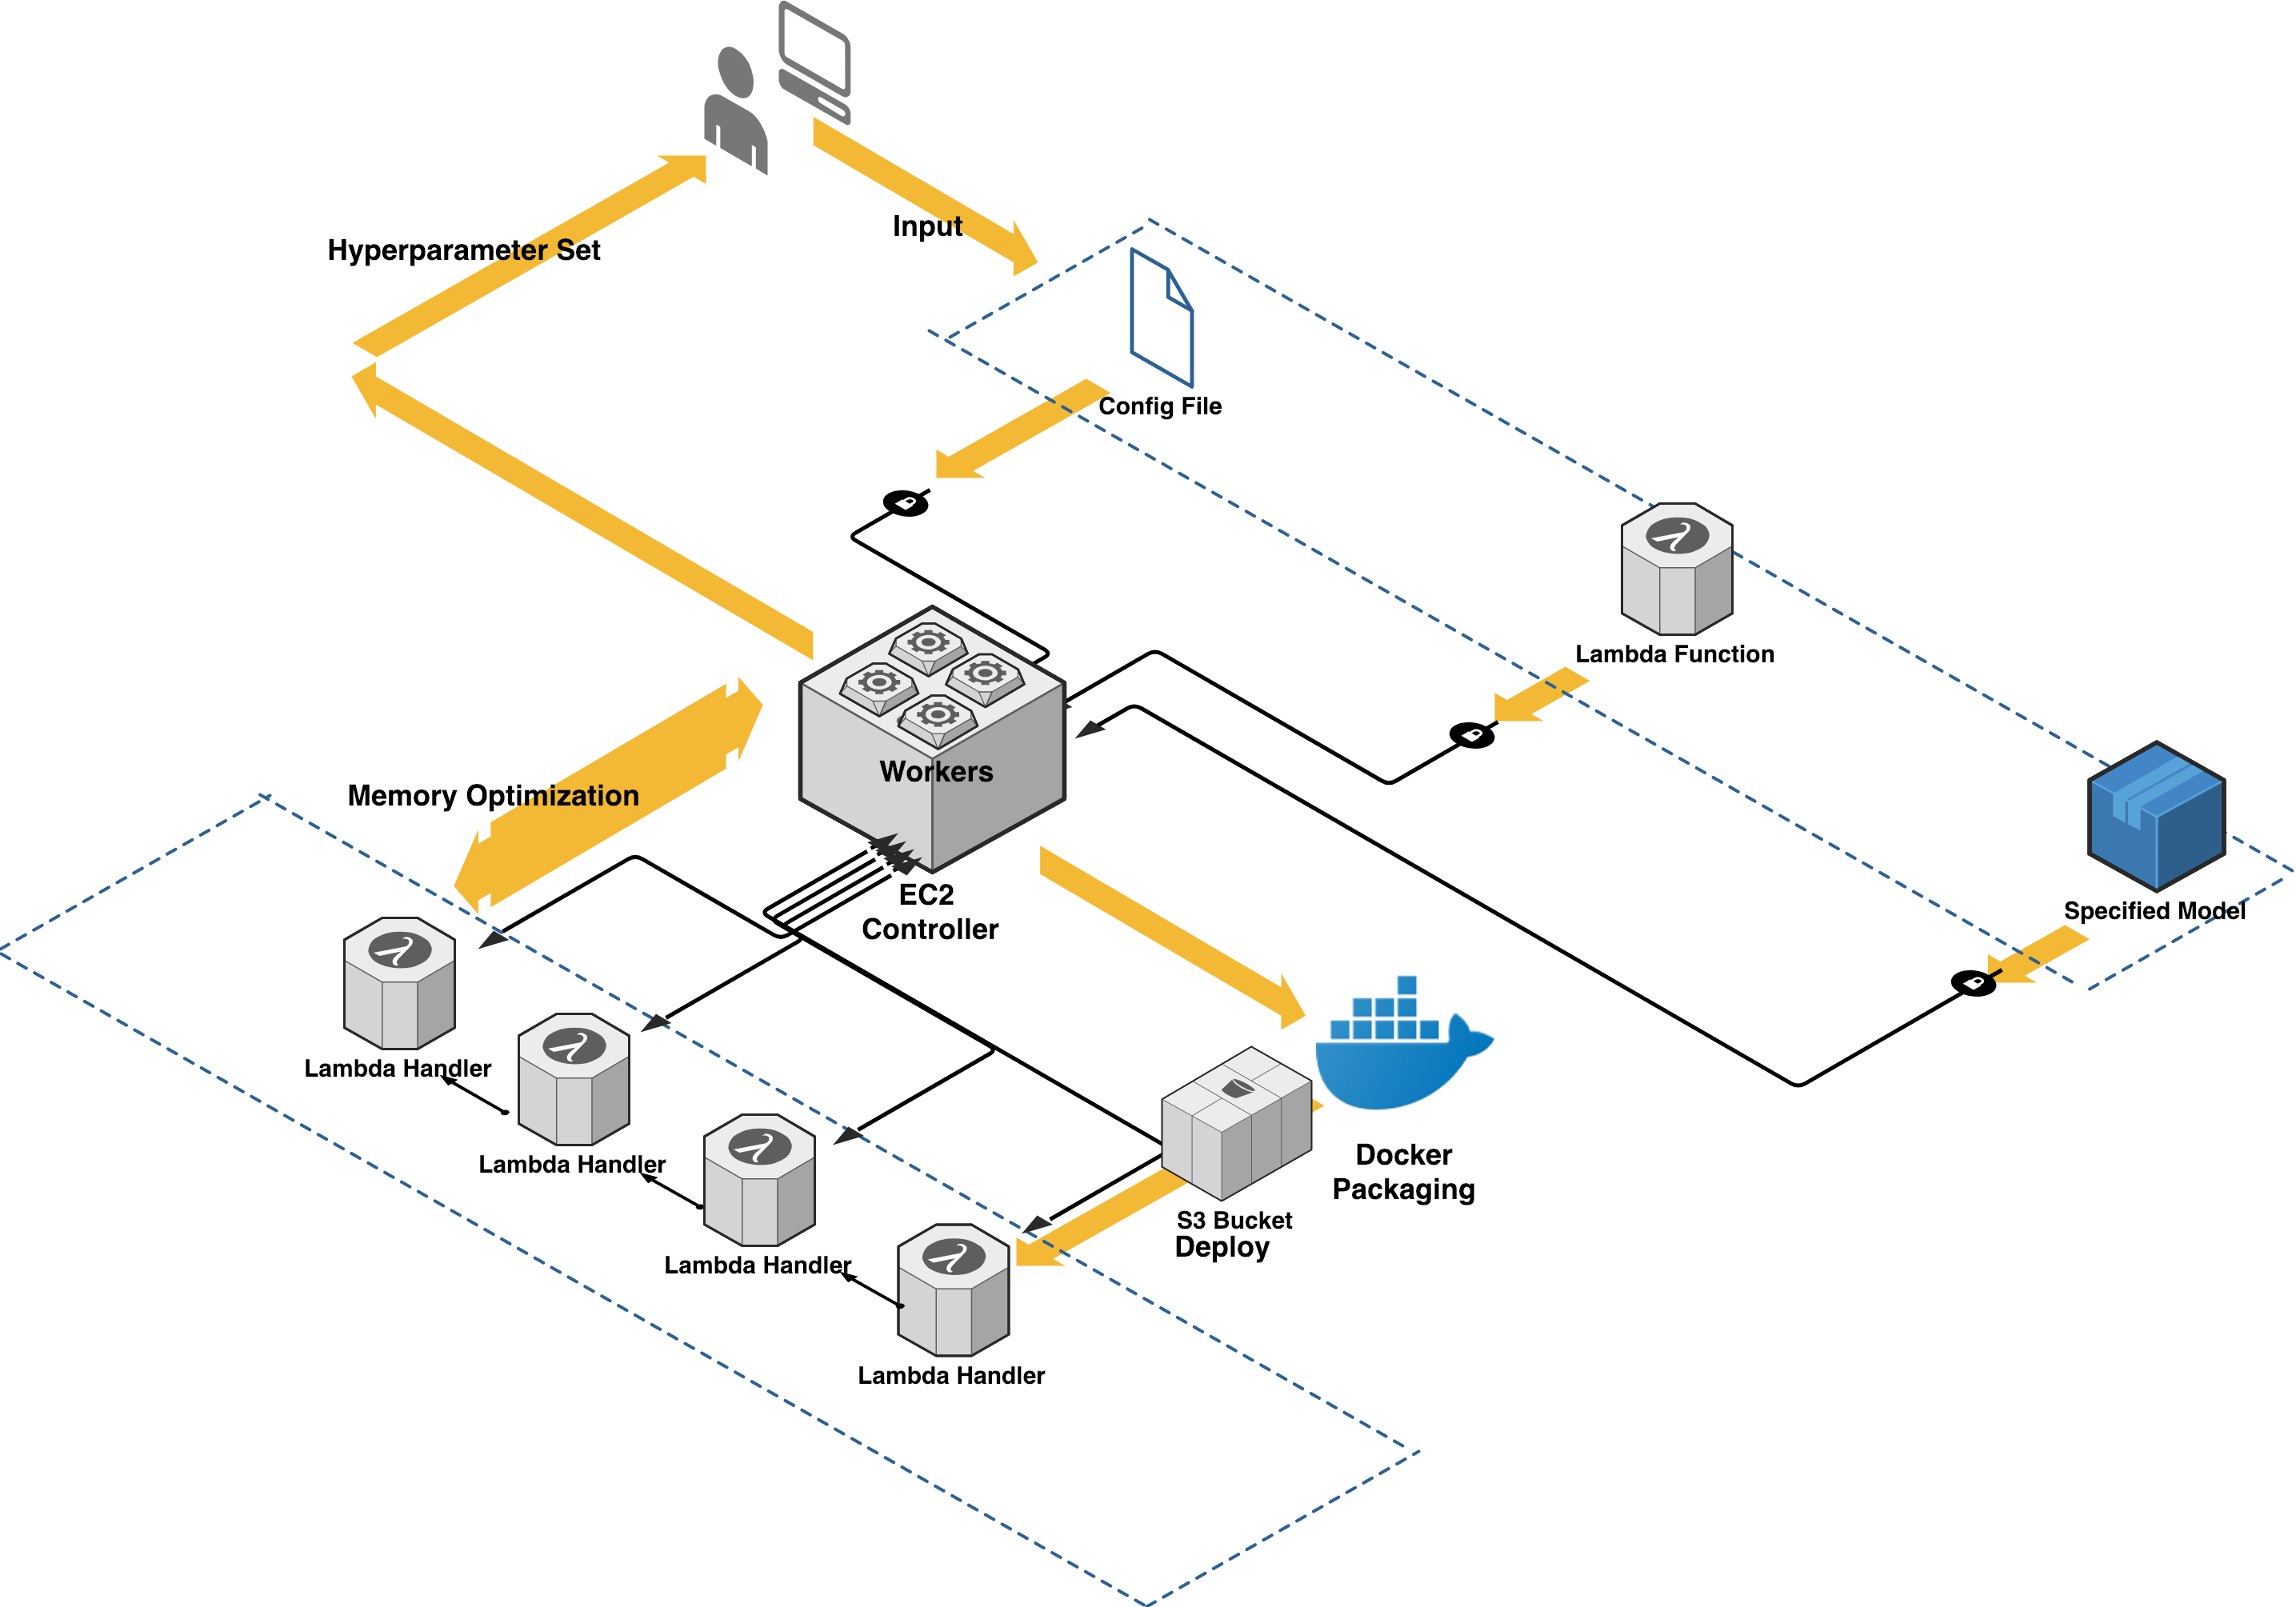
\includegraphics[scale=0.08]{Seneca}
\caption{The Seneca Architecture.
%Users specify hyperparameter options in the configuration file and provides lambda function. Seneca automatically package, deploy and optimize lambda function on AWS before completing grid search process and selecting best hyperparameter setting.
\label{fig:seneca}}
\vspace{-0.2in}
\end{figure}

To facilitate model search and selection using the serverless
architecture, we have developed Seneca, a framework for tuning the
hyperparameters of machine learning applications in AWS Lambda.  The
Seneca pipeline consists of packaging, deployment, function
optimization, and hyperparameter tuning. Figure~\ref{fig:seneca} shows
the architecture of Seneca.  In the the upper-right-front, we show the
three inputs that Seneca expects from its users: (\textit{A}) a
hyperparameter configuration file, (\textit{B}) a dataset URL, and
(\textit{C}) the lambda function of the machine learning
application. The configuration file specifies a set of values for
each hyperparameter that the application expects. Seneca creates the
Cartesian product of all options in this configuration as
the search space. The dataset URL refers to a valid dataset stored in
the AWS Simple Storage Service (S3)~\cite{ref:awss3}.
%\footnote{\url{https://aws.amazon.com/s3/}}.

Based on the specified machine learning application, Seneca
automatically builds and deploys an AWS Lambda application by
launching a Docker container that mirrors the AWS Lambda execution
environment, checks and installs the machine learning application and
any libraries it requires, compresses the application and uploads it
to S3 (a
work-around for the 10MB AWS Lambda function size restriction).
Seneca constructs an AWS Lambda function from a template that, when
executed, will download the dataset and split it into a training and
testing set, and construct, test, and evaluate a model using the
application and a set of hyperparameter values passed in by Seneca as
arguments.  Users can specify the train/test split ratio that should
be used by Seneca; the default is 80\%/20\% for classification tasks.  The function returns a
testing score.  Upon completion of this process, the container deploys
the function to AWS Lambda using the AWS Command Line
Interface~\cite{ref:awscli}
%\footnote{\url{https://aws.amazon.com/cli/}} 
and the developers credentials.



\subsection{Optimizing Memory Use}

The cost of using AWS Lambda (i.e. \texttt{compute charge}) 
is the billed duration (execution time rounded up to the
nearest 100ms)~\cite{ref:pricing}
%~\footnote{\url{https://aws.amazon.com/lambda/pricing/}}
multiplied by the allocated memory of each invoked function.
One goal of our work is to optimize memory use of these
applications in order to reduce cost, and to investigate
the trade-offs of doing so.

Currently, allocated memory for a Lambda function can be set
from 128MB to 3008MB in increments of 64MB.
AWS documentation~\cite{ref:lambdalimits}
%~\footnote{\url{https://docs.aws.amazon.com/lambda/latest/dg/resource-model.html}} 
states that Lambda allocates CPU to functions  corresponding to allocated memory size,  
as is done for general purpose AWS EC2 instance types.

\begin{figure}[t] \centering 
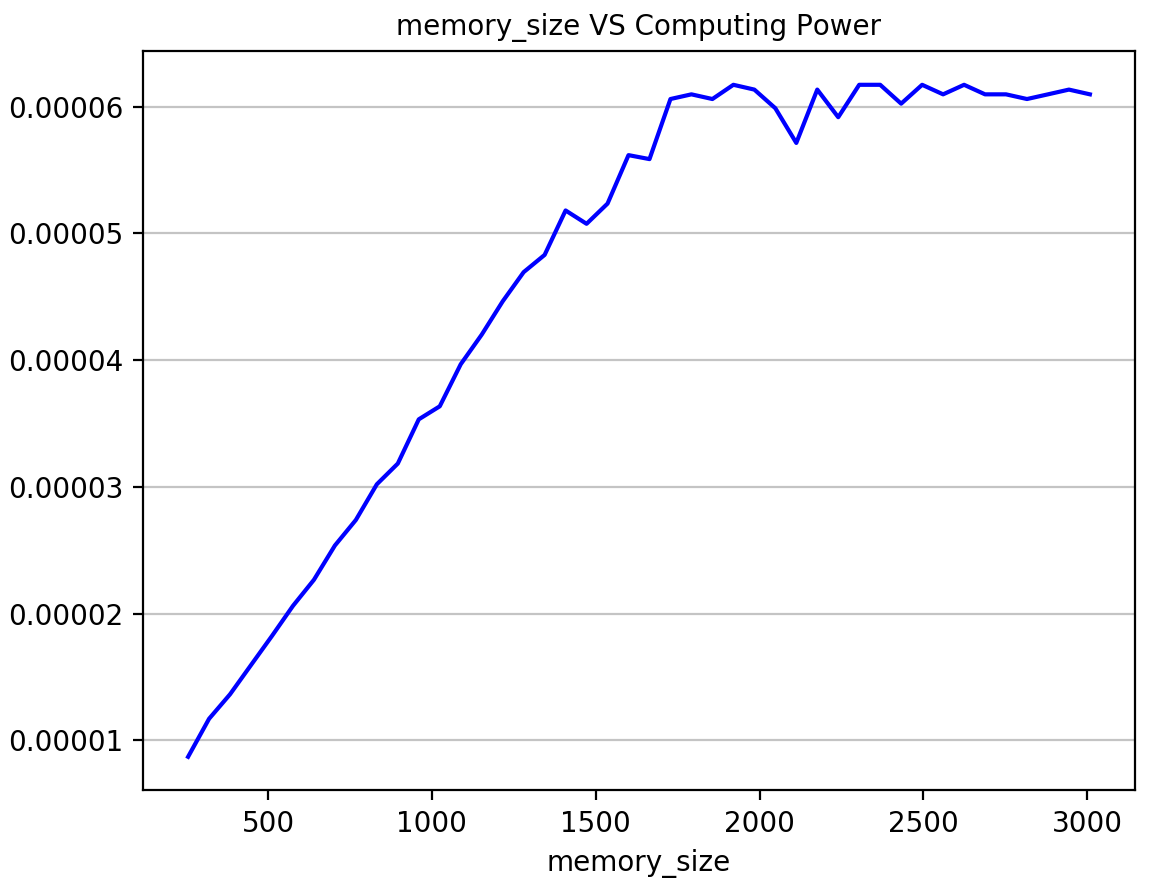
\includegraphics[scale=0.5]{memory}
\caption{The relationship between allocated memory and reciprocal of billed duration, which represents compute power for a compute-bound Lambda function.
\label{fig:memory}}
% \vspace{-0.2in}
\end{figure}

\begin{figure}[t] \centering 
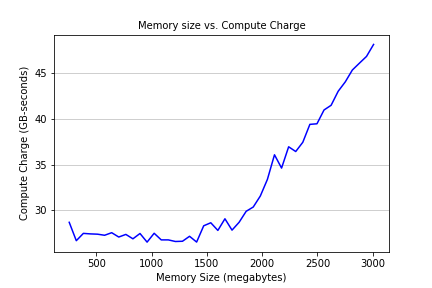
\includegraphics[scale=0.5]{compute_charge}
\caption{The relationship between allocated memory and compute charge for a compute-bound Lambda function.
\label{fig:compute_charge}}
% \vspace{-0.2in}
\end{figure}


To evaluate the relationship between memory, CPU, and cost, 
we analyze a 3-D matrix multiplication serverless benchmark~\cite{ref:matrix} using AWS Lambda.
We configure different functions to use each of the 46 possible allocated memory 
options.  Figure~\ref{fig:memory} shows the relationship between allocated memory 
(x-axis) and reciprocal of billed duration (y-axis). 
Figure~\ref{fig:compute_charge} shows the relationship between memory 
size (x-axis) and compute charge (y-axis). 
We observe that for this benchmark, billed duration 
plateaus after 1600 MB, at which point compute charge increases.
That is, we achieve no further execution time benefit (only cost increase)
after this point.

We use this relationship within
Seneca to optimize its cost (\texttt{compute charge}) via an extension
that enables it to automatically identify the appropriate
setting for allocated memory for each application.
However, instead of exhaustively testing all 46 possible 
memory configurations as we did for the matrix benchmark, 
which may be costly,  Seneca employs the heuristic outlined in
Algorithm~\ref{algo:optimizer}. 

The Seneca optimizer first configures and invokes the function using a user-defined payload.  From this run, Seneca obtains the \texttt{maximum memory used}
by the function as reported by AWS Cloudwatch,
and uses it as the starting point in its search.
Seneca then defines two double-ended queues 
(\textit{deque}) of length N, to store 
\texttt{allocated memory} and \texttt{compute charge} data of different invocations. While the current 
allocated memory is less than or equal to 3008 MB, 
the optimizer reconfigures and invokes the function 
using the next increment for memory allocation.  It 
calculates the compute charge for each invocation 
using current allocated memory and billed duration. 

We employ two exit conditions. The first is when the  compute charge monotonically increases across \textit{deque}. The second is when the increase in slope is greater than a threshold. When the optimizer finds that both conditions hold, it pops the left-most value from \textit{deque} and configures the function to use that value for allocated memory for all future invocations. If these two conditions can not be satisfied during search, the allocated memory will be configured as the memory size that results in minimal compute charge within the \textit{deque}. After extensive experimentation, we find that $N=5$ and a slope threshold of 1 work best, but these values are configurable. In addition, this optimization can be turned on or off via a command line argument to Seneca.

\begin{algorithm}[]
\caption{Seneca Optimizer Heuristic}
\label{algo:optimizer}
\SetAlgoLined
\KwData{Typical payload}
\KwResult{Optimal allocated memory}
Find memory used by payload as starting point\;
Define deque for allocated memory \& compute charge\;
 \While{allocated memory $\leq$ 3008 MB}{
  \eIf{compute charge monotonically increases in deque \& slope $\geq$ threshold}{
   popleft from deque\;
   configure allocated memory as optimum\;
   exit()\;
   }{
   increase allocated memory by 64 MB\;
   probe lambda function\;
   append memory and compute charge to deque\;
  }
 }
\end{algorithm}

\subsection{Tuning Process}

To facilitate parallel function invocation, Seneca integrates 
Celery~\cite{ref:celery}.
%\footnote{\url{http://www.celeryproject.org/}}
Celery is an asynchronous task queue 
that uses distributed message passing. Celery workers are processes 
that take tasks from the queue, execute the tasks with the arguments specified, 
and store the result that is returned 
in a database (we use Redis~\cite{ref:redis}
%~\footnote{\url{https://redis.io/}} 
in our prototype). 

Based on the configuration file, Seneca creates and enqueues a list of
payloads (function arguments) for each combination of hyperparameter
values.  The Seneca celery workers invoke the application's Lambda
function by each payload for model construction. Upon function
termination, the worker records a score for the hyperparemeter
configuration in the database.  When the queue is drained and all
workers have completed, Seneca extracts and reports the best score,
configuration, and model from the database. Users can then use the
model for inference given other datasets without retraining to
amortize the time/cost of Seneca.
% Users can then evaluate the prediction power of the models (using Seneca if desired) 
% for other datasets without retraining to amortize the time/cost of Seneca.


We assume that the dataset supplied to Seneca by the user is representative of 
datasets on which the 
resulting model will be used.  
%In addition, we use prediction error as the 
%score (i.e., mean squared error for regression and accuracy percentage for classification) 
%instead of $R^2$, which describes explanatory power, to avoid overfitting.
As part of future work, we are considering using multiple datasets and a ranges
of hyperparameter values to preclude the need for users to specify
them and to consider a wider range of values.

\section{Evaluation}

\label{sec:eval}

\begin{table}[t]
\centering
%\scriptsize
%\resizebox{\columnwidth}{!}{
\begin{tabular}{|l|l|} \hline
\textbf{Application}& \textbf{Description}\\
\hline
Prophet& Time series decomposition and prediction\\ 
\hline
Multi-Regression& Multiple linear regression/prediction of time series\\
\hline
XGBoost& Regression and classification by gradient boosting\\
\hline
SVC & Classification based on support vector machine\\
\hline
NN& Classification by layered artificial neural network\\
\hline
\end{tabular}
%}
\caption{Machine learning applications used 
to evaluate Seneca. 
%paper submission is blind (so such references must be omitted so as not to reveal our identities):
%Code base is available at project repository~\cite{ref:seneca}.
\label{tab:bmarks}}
\vspace{-0.1in}
\end{table}

\begin{table}[t]
\centering
% \scriptsize
%\resizebox{\columnwidth}{!}{
\begin{tabular}{|l|l|l|} 
\hline
\textbf{Hyperparameter}& \textbf{Default} & \textbf{Tuning options}\\
\hline
growth & linear & [linear, logistic] \\
\hline
changepoint prior scale & 0.05 & [0.05, 0.5] \\
\hline
holidays prior scale & 10 & [1, 5, 10] \\
\hline
seasonality prior scale & 0.5 & [0.1, 0.5] \\
\hline
fourier order & 10 & [5, 10, 15, 20] \\
\hline
seasonality mode & additive & [additive, multiplicative] \\
\hline
interval width & 0.8 & [0.5, 0.8] \\
\hline
\end{tabular}
%}

\caption{Hyperparameters Seneca considers for \textbf{Prophet}. 
\label{tab:prophet_para}}
%\vspace{-0.1in}
\end{table}

\begin{table}[t]
\centering

\begin{tabular}{|l|l|l|} 
\hline
\textbf{Hyperparameter}& \textbf{Default} & \textbf{Tuning options}\\
\hline
%hidden layer size & 100 & [100] \\
%\hline
max depth & 3 & [3, 4]\\
\hline
learning rate & 0.1 & [0.1, 0.01] \\
\hline
N estimators & 100 & [100, 400] \\
\hline
objective & reg:linear & [reg:linear, rank:pairwise] \\
\hline
booster & gbtree & [gbtree, gblinear, dart] \\
%\hline
%n jobs & 1 & [1,4]\\
%\hline
%gamma & 0 & [0,0.01] \\
\hline
min child weight & 1 & [0.1, 1] \\
\hline
scale positive weight & 1& [1, 2] \\
%\hline
%sample tree & 1& [0.2,0.5,1]\\
%\hline
%samp level & 1& [0.2,0.5,1]\\
%\hline
%ralpha & 0& [0.0.1,0.9] \\
%\hline
%rlambda & 1& [0.1,0.9,1] \\
\hline
base score & 0.5 & [0.5, 10] \\
\hline
%random state & 123& [123] \\
%\hline
\end{tabular}

\caption{Hyperparameters Seneca considers for \textbf{XGBoost}. 
\label{tab:xgboost_para}}
\vspace{-0.2in}
\end{table}

\begin{table}[t]
\centering
%\scriptsize

\begin{tabular}{|l|l|l|} 
\hline
\textbf{Hyperparameter}& \textbf{Default} & \textbf{Tuning options}\\
\hline
C & 1.0 & [0.5, 1.0] \\
\hline
kernel & rbf & [rbf, linear, poly, sigmoid] \\
\hline
degree & 3 & [3, 4] \\
\hline
gamma & auto& [auto, scale] \\
\hline
coef0 init & 0.0 & [0.0, 1.0] \\
\hline
%shrink & True & [True] \\
%\hline
probability & False & [False, True] \\
\hline
tol & 1e-3& [1e-3, 1e-4] \\
\hline
%cache & 5.0& [5.0] \\
%\hline
%max iter & 20 & 20 \\
%\hline
decision function shape & ovr & [ovo, ovr] \\
\hline
%random state & 123& [123] \\
%\hline
\end{tabular}

\caption{Hyperparameters Seneca considers for \textbf{SVC}. 
\label{tab:svc_para}}
%\vspace{-0.2in}
\end{table}

\begin{table}[t]
\centering
%\scriptsize

\begin{tabular}{|l|l|l|} 
\hline
\textbf{Hyperparameter}& \textbf{Default} & \textbf{Tuning options}\\
\hline
%hidden layer size & 100 & [100] \\
%\hline
activation & relu & [identity, tanh, relu] \\
\hline
solver & adam & [lbfgs, sgd, adam] \\
%\hline
%alpha & 0.0001 & [0.0001] \\
%\hline
%batch size & auto & [200,auto] \\
\hline
learning rate & constant & [constant, invscaling, adaptive] \\
\hline
learning rate init & 0.001 & [0.001, 0.0001] \\
\hline
power T & 0.5 & [0.1, 0.5] \\
%\hline
%max iter & 20& [20] \\
%\hline
%shuffle & True& [True] \\
%\hline
%random & 123& [123] \\
\hline
tol & 1-e4 & [1e-4, 1-e5] \\
%\hline
%momentum & 0.9& [0.9] \\
%\hline
%early stop & False& [False] \\
%\hline
%beta1 & 0.9& [0.9] \\
%\hline
%beta2 & 0.999& [0.999] \\
%\hline
%epsilon & 1e-8& [1e-8] \\
\hline
n iter no change & 10 & [10, 20] \\
\hline
\end{tabular}

\caption{Hyperparameters Seneca considers for \textbf{NN}.
\label{tab:nn_para}}
\vspace{-0.2in}
\end{table}

In this section, we empirically evaluate Seneca in terms of machine learning (ML) 
model output quality, performance, and cost.
We first overview the ML applications 
that we consider and our experimental methodology. 
We then present our results. 

\subsection{Benchmark Applications and Training/Testing Datasets}
The ML applications that we use to evaluate Seneca 
are described in Table~\ref{tab:bmarks}.
Prophet, Multi-Regression, and XGBoost are regression
applications; 
XGBoost, SVC, and NN are classification applications (XGBoost 
implements both regression and classification tasks).
The regression applications compute the mean square error (MSE) 
as $\frac{1}{n}\sum_{i=1}^{n}(Y_i - \hat{Y_i})$, where $\hat{Y_i}$ is the ground truth, 
$Y_i$ is model prediction and n is the number of data points. The applications
return the average MSE across cross validations.
The classification applications compute and return a classification accuracy 
percentage, which is calculated
as $\frac{1}{n}\sum_{i=1}^{n}1(Y_i = \hat{Y_i})$, where $Y_i$ is the
prediction class, $\hat{Y_i}$ is the true class, $n$ is the number of samples, and 1(x) is the indicator function. 

Prophet~\cite{ref:prophet} is an open source time series analysis library developed
by Facebook.  The input dataset we consider is a time series of view counts
of Peyton Manning's Wikipedia page (Dec. 2007--Jan. 2016).
The dataset exhibits both seasonality and a holiday effect (e.g. around 
super bowl games).  We use the first 6 years as the training set 
and the last 2 years as the testing set.  We use a cross-validation 
horizon (sliding window) of 1-year, and a period (sliding pace) 
of 180 days.  As such, Seneca performs three cross-validations for 2-year test range.

Prophet expects multiple hyperparameters.
\textit{growth} specifies linear or logistic trend model growth and \textit{prior scale} indicates the strength of the sparse prior probability. There are three prior scale hyperparameters for change point, holidays, and seasonality. Since Prophet uses a Fourier sum to estimate seasonality, the \textit{fourier order} is the number of terms in the partial Fourier sum. \textit{Seasonality mode} indicates that the effect of seasonality is either multiplicative or additive. Finally, the width of uncertainty intervals is set using \textit{interval width}.

Each application has default hyperparameter settings (i.e. default values or those recommended by the application maintainer). The hyperparameters, their default and optional values that we consider for Prophet are listed in the Table \ref{tab:prophet_para}.

Multi-Regression is a regression application developed by others as part of
an Internet-of-Things (IoT) project~\cite{iot-cpu} (which has been
extended from linear regression described in the citation 
to multiple linear regression by the authors of this prior work).
The application uses multiple linear regression models
to predict outdoor temperature from the processor 
temperature of single board computers (SBCs).  
The training dataset consists of eight input time 
series (one per SBC, each containing 
5-minute measurements) from Apr. 5th to Dec. 10th, 2018.

Hyperparameter configuration for Multi-Regression is a subset of input SBC time series.
Seneca considers all \texttt{$2^N - 1$} potential subsets (for $N$ input time series).
For this application, the default parameterization is the 
full set of input time series (8 in this case).
The test dataset is a time 
series of the outdoor temperature (ground truth) 
over the same period.  
The application makes 
predictions for each of these outdoor temperatures
using the regression coefficients constructed from the training set
for each new value in the test set.
%and computes and returns the MSE between predicted 
%and ground truth value pairs.

XGBoost~\cite{ref:xgboost-web}, SVC~\cite{ref:svc}, and NN~\cite{ref:neural_network} 
are the classification applications that we consider.
XGBoost~\cite{ref:xgboost-web} is an open source 
framework for gradient boosting, which 
performs both regression and classification. 
The hyperparameters and their default values 
are listed in Table~\ref{tab:xgboost_para}, their definitions can be
found in~\cite{ref:xgboostparams}. SVC uses support vector machines to implement classification as part of the libsvm~\cite{ref:libsvm} library.
The hyperparameters and their defaults that Seneca uses for SVC in this study are listed in Table~\ref{tab:svc_para} with definitions
in~\cite{ref:svcparams}. NN is a machine 
learning application leveraging neural network to identify patterns from an input dataset. 
Here we implement a feed-forward multi-layer perceptron model~\cite{ref:feedforward_nn} 
for classification. The hyperparameters and their defaults for NN are listed in Table~\ref{tab:nn_para} with definitions
in~\cite{ref:nnparams}. 
%\footnote{\url{https://scikit-learn.org/stable/modules/generated/sklearn.neural_network.MLPClassifier.html}}.
%\footnote{\url{https://xgboost.readthedocs.io/en/latest/python/python_api.html\#module-xgboost.sklearn}}
%\footnote{\url{https://scikit-learn.org/stable/modules/generated/sklearn.svm.SVC.html}}

For these classification applications, we use a labeled
dataset for training, testing, and evaluation from another IoT 
project~\cite{blind}. The dataset contains measurements of individual
citrus fruit (e.g. oranges, mandarins, lemons, etc.) taken by a fruit sorting
and grading device using a large number of sensors. The measurements (i.e. features) include size, shape, weight, color, diameter, flatness, among other characteristics, for each fruit.  
The dataset has been filtered to remove correlated
features (those with an absolute value of the Pearson correlation coefficient
greater than 0.8). The dataset has been balanced by 
down-sampling and the resulting 
dataset contains 33926 rows (individual fruit) 
distributed evenly across 5 targets. Each row has
18 features.  The label identifies the field from which the individual fruit was harvested.

The applications train a model on a random subset (80\%) of the data. Each then uses this model to predict the field from which each fruit originates for the remaining 20\%. To study the impact of random data split, we consider multiple 80\%/20\% splits in our evaluation.
\subsection{Empirical Methodology}

To evaluate Seneca, we measure model output quality, execution time, memory use, and monetary cost.  For output quality (prediction accuracy) our metrics are mean squared error (MSE) for regression and percentage accuracy for classification as described above. We score model prediction accuracy and not explanatory power ($R^2$) to avoid overfitting. 

\ignore{Seneca is able to compare models for each type of application using these scores because it uses the same total number of hyperparameters for each model. Thus, the penalty function in terms of Bayesian Information Criteria is the same. 
comments: BIC is based on parameters, not for hyperparameters.} 

We compare results for the default, best (Seneca's recommendation), and worst performing hyperparameter configurations for each application type. Seneca computes all possible combinations of the hyperparameter settings specified in the configuration to extract each of these results.  \texttt{default} represents results that a novice or first time user might experience when using these applications as a ``black box.''  The \texttt{worst} shows how bad the results can be when parameters are poorly tuned.  Finally, the \texttt{best} is the upper bound on what is possible from tuning the hyperparameters for the values and datasets specified  (e.g. using expert knowledge or Seneca). 

Seneca deploys the applications automatically over AWS Lambda
and extracts execution time and memory use from 
AWS CloudWatch~\cite{ref:awscloudwatch} logs.
We compute monetary cost using the AWS Lambda pricing model~\cite{ref:pricing}.
Each function downloads the training/testing dataset 
of the application from AWS S3 upon function invocation. 
We do not consider the cost of dataset storage 
in our cost computations (it is very small).
%\footnote{\url{https://aws.amazon.com/cloudwatch/}}
%\footnote{\url{https://aws.amazon.com/lambda/pricing/}}
We also evaluate Seneca's automatic memory optimization capabilities.  To
do so we compare the execution performance and cost of the applications using
the maximum allocatable memory size to the performance and cost when run with
Seneca's automatically determined memory size. Even though \texttt{maximum memory used} reported by AWS CloudWatch can fluctuate, we 
have verified that the optimized allocated memory is sufficient for all 
hyperparameter configurations to complete successfully.  We have also verified
that the memory requirements across hyperparemeter settings do not vary 
significantly. We plan to consider applications for which hyperparameter settings require
different maximum memory sizes as part of future work.


\subsection{Application Efficacy}

\begin{table}
\centering
\begin{tabular}{|c|c|c|c|}
\hline
& Prophet & Multi-Regression & XGBoost\\
\hline
\# of Combinations & 384 & 255 & 768\\
\hline
\hline
Default MSE & 0.284 & 11.446 & 0.119 \\
\hline
Worst MSE & 1.266 & 43.752 & 8.98 \\
\hline
Best MSE (Seneca) & 0.220 & 9.621 & 0.044 \\
\hline
%percent difference between default and best 26.07%, 15.94%, 67.30%
%percent difference between worst and best 82.63%, 78.01%, 95.52%
%\begin{figure}[t] \centering 
%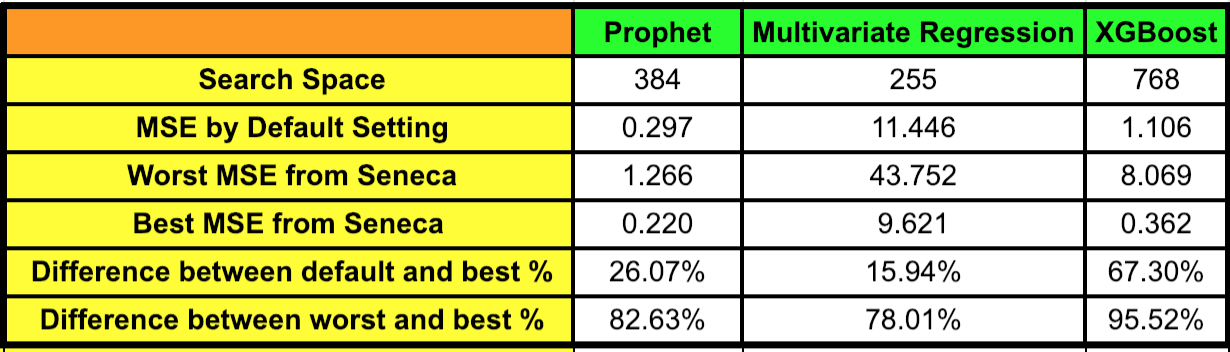
\includegraphics[scale=0.4]{mse}
\end{tabular}

\caption{Hyperparameter configuration count and MSE for the default, 
best (Seneca's recommendation), and worst configurations for the three regression applications. 
For the MSE  values (rows 3-5), lower is better.
\label{tab:mse}}
\vspace{-0.2in}
\end{table}

\begin{figure}[t] \centering 
\vspace{-0.5in}
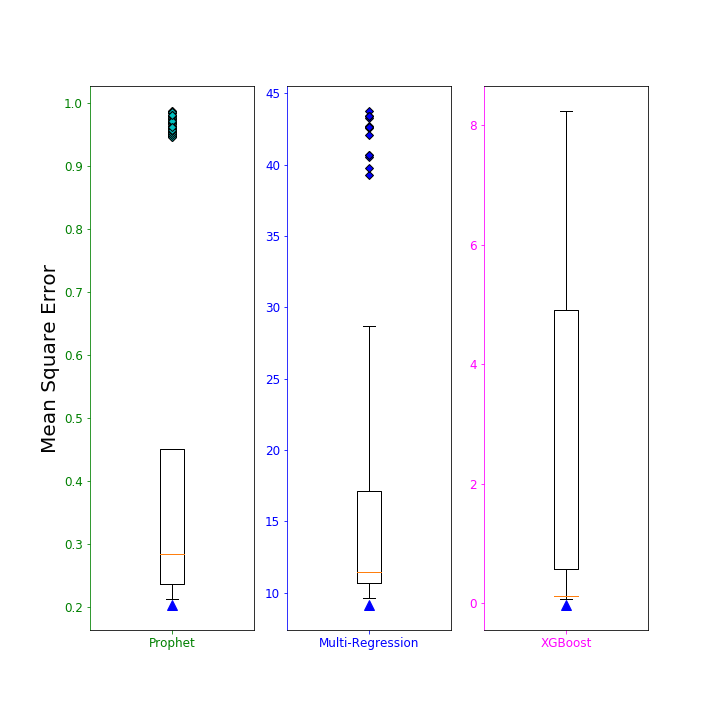
\includegraphics[scale=0.36]{box_plot_mse}
\caption{Box plot of MSE from the three regression applications across the 
hyperparameter tuning search space. The red notch shows the MSE from the default settings. 
The colored diamonds are outliers beyond two interquartile ranges. 
Seneca selects the points indicated by blue triangle.
Lower MSE values are better. 
\label{fig:box_plot_mse}}
\vspace{-0.2in}
\end{figure}

We first evaluate the quality of the output generated by each
ML applications when Seneca determines the hyperparameter settings. We
first show the results for the regression applications in
Table~\ref{tab:mse}.
The first row of data is the number of hyperparameter 
configurations that Seneca considers for each.
The last three rows show the MSE for the default, worst, and best performing (Seneca's recommendation)
hyperparameter configuation (lower is better).
Seneca reduces MSE by 22.56\%, 15.94\%, and 44.88\%, for Prophet, Multi-Regression, and XGBoost,
respectively, for the datasets and training methodologies that we consider.
Verses the worst case, Seneca reduces MSE by 82.62\%, 78.01\%, and 99.28\%, respectively.

Figure~\ref{fig:box_plot_mse} shows the MSE box plot for the hyperparameter search space for these applications (lower is better). 
The central rectangle covers the interquartile range (IQR),
which is defined as the range of data
points from first quartile to third quartile \texttt{$(Q3 - Q1)$}.
The upper whisker extends to the last datum less
than \texttt{$(Q3 + 2 * IQR)$} and the lower whisker extends to the first datum greater
than \texttt{$(Q1 - 2 * IQR)$}. The data points beyond the whiskers are considered outliers
and are plotted as colored diamonds. The red notch identifies the MSE that results from training
the model using the default settings of hyperparameter.
The blue triangle identifies the MSE of Seneca.
The difference between red notch and blue triangle
is the improvement brought about by the use of Seneca, over 
using the default parameter setting.
The plot also shows
that Prophet and Multi-Regression have a significant number of outliers,
indicating that a comprehensive search is critical to finding the best configurations.

%%%%%%%%%%%%%%%%%%%%% classification apps - ML model output quality %%%%%%%%%%%%%%%%%%%%%%%%%
\begin{table}
\centering

\begin{tabular}{|l|c|c|c|}
\hline
\textbf{80\%-20\%} & XGBoost & SVC & NN\\
\hline
\# of Combinations & 768 & 512 & 432 \\
\hline
\hline
Default Accuracy & 95.65\% & 21.77\% & 79.53\%\\
\hline
Worst Accuracy&0.00\%&14.08\% & 19.40\%\\
\hline
Best Accuracy (Seneca) &98.11\% & 40.81\% & 83.31\%\\
\hline
%\hline
%\hline
%\textbf{20\%-80\%} & XGBoost & SVC & NN\\
%\hline
%Default Accuracy & 95.07\% & 21.31\% & 55.44\%\\
%\hline
%Worst Accuracy&0.00\% & 9.42\% & 19.55\%\\
%\hline
%Best Accuracy (Seneca) & 98.68\% & 43.61\% & 60.89\%\\
%\hline
%\hline
%\textbf{0.1\%-99.9\%} & XGBoost & SVC & NN\\
%\hline
%Default Accuracy & 86.37\% & 20.02\% & 20.00\%\\
%\hline
%Worst Accuracy & 0.00\% & 19.99\% & 19.79\%\\
%\hline
%Best Accuracy (Seneca) & 89.14\% & 55.79\% & 29.99\%\\
%\hline

%percent difference between default and best 83.65%, 83.84%, 79.83%
%percent difference between worst and best 86.07%, 85.73%, 84.63%
%\begin{figure}[t] \centering 
%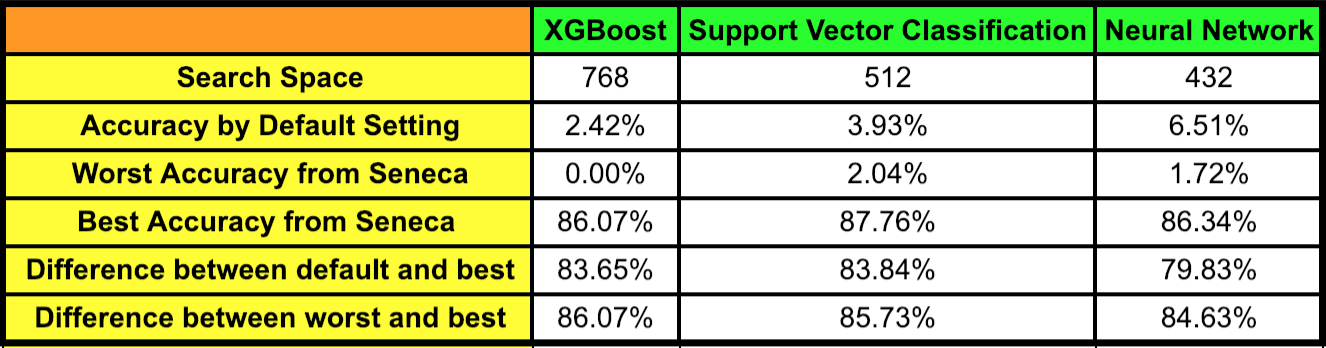
\includegraphics[scale=0.38]{accuracy}
\end{tabular}

\caption{Accuracy for the 
default, best (Seneca's recommendation), and worst hyperparameter configurations for 
the three classification applications using 80\% of the data to train and 20\%
of the data as a test set. Higher accuracy is better.
\label{tab:accuracy}}
\vspace{-0.1in}
\end{table}

\begin{figure}[t] \centering 
\vspace{-0.1in}
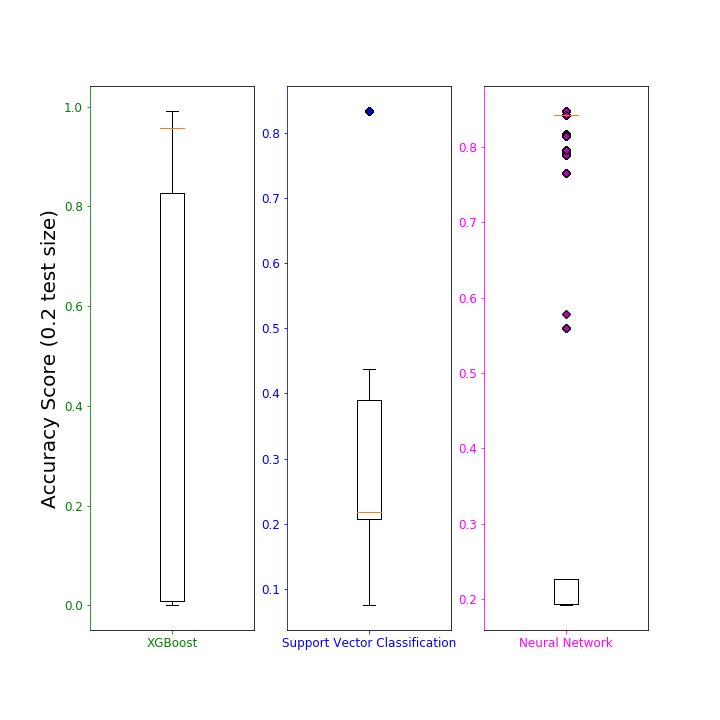
\includegraphics[scale=0.36]{box_plot_Accuracy_20}
\vspace{-0.4in}
\caption{Box plot of accuracy reported for three classification applications across 
the hyperparameter search space. The red notch indicates the accuracy that results
from default hyperparameter values.
The diamonds are outliers beyond two interquartile ranges. 
Seneca selects the points indicated by blue triangle. 
Higher accuracy is better. 
\label{fig:box_plot_accuracy}}
\vspace{-0.2in}
\end{figure}

\begin{table}[t]
\centering
\scriptsize
% \scriptsize
% \resizebox{\columnwidth}{!}{

\begin{tabular}{|l|c|c|c|} 
\hline
 & \textbf{Exec Time (Secs)} & \textbf{Memory Use (MB)} & \textbf{Best Accuracy}\\
\hline
\hline
XGBoost\_1 & 1244.42 (32.58) & 228.74 (15.92) & 99.13\% \\
\hline
XGBoost\_2 & 1280.56 (38.47) & 225.10 (19.67) & 97.70\% \\
\hline
SVC\_1 & 116.73 (1.11) & 224.44 (19.64) & 40.81\% \\
\hline
SVC\_2 & 115.33 (3.96) & 228.55 (16.20) & 44.11\% \\
\hline
NN\_1 & 116.10 (6.05) & 328.84 (16.40) & 83.31\% \\
\hline
NN\_2 & 121.29 (2.18) & 327.57 (16.44) & 83.92\% \\
\hline

\end{tabular}
%}

\ignore{ %the below has errors
% \scriptsize
% \resizebox{\columnwidth}{!}{

\begin{tabular}{|l|c|c|c|} 
\hline
 & \textbf{Exec Time (Secs)} & \textbf{Memory Use (MB)} & \textbf{Best Accuracy}\\
\hline
\hline
XGBoost\_1 & 1244.42 (32.58) & 228.74 (15.92) & 99.13\% \\
\hline
XGBoost\_2 & 1280.56 (38.47) & 225.10 (19.67) & 97.70\% \\
\hline
SVC\_1 & 116.73 (1.11) & 224.44 (19.64) & 40.81\% \\
\hline
SVC\_2 & 115.33 (3.96) & 228.55 (16.20) & 44.11\% \\
\hline
NN\_1 & 116.10 (6.05) & 328.84 (16.40) & 83.31\% \\
\hline
NN\_2 & 121.29 (2.18) & 327.57 (16.44) & 83.92\% \\
\hline

\end{tabular}
%}
}

\caption{The mean and standard deviation (in parentheses) for execution time and memory use 
(across 30 runs),
and best accuracy score for the classification applications using two different random splits. 
\label{tab:exec_memory}}
\vspace{-0.1in}
\end{table}


We next empirically evaluate Seneca's model output quality for the three
classification applications: XGBoost (classification), SVC, and NN.
Table~\ref{tab:accuracy} presents the accuracy percentage (higher is better)
for each application (3 right-most columns)
for the default, worst, and best (Seneca's recommendation) hyperparameter tuning
configurations (data rows 2-4).
The first row 
reports the number of configurations that Seneca considers in its search space.
Using a random 80/20 (train/test) percent split,
Seneca increases accuracy by 2.46\%, 19.04\%, and 3.79\%, for XGBoost
(classification), SVC, and NN applications, respectively.  
Because XGBoost and NN use a well-tuned default parameter set that works well for most datasets, Seneca provides only modest improvements.
Compared to the worst case however, Seneca improves accuracy by 98.11\%, 26.74\%, and 64.17\%,
respectively.  

Figure~\ref{fig:box_plot_accuracy} presents the accuracy box plot across the hyperparameter search space for these applications (higher is better).  
The central rectangle covers the first-third quartile
\texttt{$(Q3 - Q1)$} and the whiskers span from \texttt{$(Q3 + 2 * IQR)$} to \texttt{$(Q1 - 2 * IQR)$}.
The red notch indicates the accuracy metric from the model trained using the default
settings and colored diamonds show outliers beyond the whiskers.
The blue triangle at the top identifies the accuracy percentage reported by Seneca.

The model output quality results across applications, show that prediction
accuracy (for a given dataset) is dramatically
affected by hyperparameter settings.  Predictably, the default settings are
near the ``good'' end of the spectrum, however, Seneca is able to find the
parameterization that improves output quality over the default settings
in each case.

To investigate the potential impact of Seneca's 80/20 percent data split for the classification
applications, we next evaluate the quality of the output generated from 
each when we consider different 80/20 random splits.
To enable this, we run Seneca 30 times to obtain execution time, memory use, 
and best accuracy score. We report the
mean and standard deviation (in parentheses) 
for execution time and memory use across runs,
and the best accuracy score in
Table~\ref{tab:exec_memory}. Each pair of rows shows the results for two different random splits.
Our earlier results use input 1; this table adds results for a second, 80/20 
random split of the input (we also considered other random splits, which we omit for brevity, 
and the results are similar).  The performance and Seneca score is similar across splits. 
This result indicates that for these applications, 
users can repeatedly employ the recommended models for inference on other datasets or splits,
to amortize the cost of using Seneca.

\subsection{Cost Analysis}

We next analyze the monetary cost incurred by Seneca with and without 
Seneca's memory optimization.
We consider the use of the maximum allocatable memory (3GB) and Seneca's 
automatic detection and configuration of allocated memory.
This optimization requires
that Seneca intelligently probe to determine the best memory size 
to use.  We report the cost of these probes as \texttt{Optimizer Cost}.

Table~\ref{tab:cost_optimized} shows the results with and without
the Seneca memory optimization for each of the five applications.
The first two rows show the results when we use the maximum allocated memory 
for the Lambda functions. We present execution time in minutes (row 1) and 
monetary cost in cents (row 2). 
Rows 3--6 show the performance and cost when using Seneca's memory optimization.
\texttt{Exec time opt} is the execution time in minutes.
\texttt{Optimizer Cost} is monetary cost in cents of Seneca's memory size detector.
\texttt{Cost opt} is monetary cost in cents of using Seneca's memory optimizer.
\texttt{Total cost} is the overall cost of using Seneca to perform hyperparameter 
tuning for these applications and datasets (sum of Optimizer Cost and Cost opt).
The last two rows show the monetary savings in cents (row 7) and percent savings (row 8)
of using Seneca's memory optimization.  Seneca's memory optimization reduces
the monetary cost of its use from 10--35\% (25\% on average).


\begin{table}
\centering
\scriptsize
\resizebox{\columnwidth}{!}{
\begin{tabular}{|l|c|c|c|c|c|}
\hline
& \textbf{Prophet} & \textbf{MR} & \textbf{XGBoost} & \textbf{SVC} & \textbf{NN} \\
\hline
\hline
Exec time max (mins)& 24.96 & 4.18 & 17.48 & 1.91 & 2.49 \\
\hline
Cost max (\$) & 0.722 & 0.121 & 0.5 & 0.023 & 0.072 \\
\hline
\hline
Exec time opt (mins)& 38.7 & 8.72 & 29.07 & 1.95 & 3.17 \\
\hline
Optimizer Cost (\$) &0.033 & 0.014 & 0.003 & 0.010 & 0.008 \\
\hline
Cost opt (\$) &0.62 & 0.086 & 0.354 & 0.007 & 0.056 \\
\hline
Total Cost (\$) &0.653 & 0.1 & 0.357 & 0.016 & 0.064 \\
\hline
\hline
Savings (\$) & 0.07 & 0.02 & 0.15 & 0.007 & 0.008\\
\hline
Savings (\%) & 10\% & 17\% & 30\% & 30\% & 11\%\\
\hline
\end{tabular}
}

\caption{Seneca Memory Optimization: Rows 1--2 show the execution time and  monetary cost 
of using Seneca without its memory optimization (allocated memory = 3G). 
Rows 3-6 is the execution time and cost, 
respectively, when using the Seneca memory optimizer. 
Rows 7-8 show the savings in cents and percentage, respectively.
\label{tab:cost_optimized}}
%\vspace{-0.1in}
\end{table}

Table~\ref{tab:cost_optimized} illustrates two important points.
First, using AWS Lambda, full hyperparameter space exploration is inexpensive in
\textit{absolute} dollar cost terms and Seneca's automatic memory size optimization
decreases this cost further.  Second, memory optimization reduces cost but can 
increase the total execution time for parameter search 
since the functions must operate under additional memory 
constraints (versus using the maximum allocated memory).  
In addition, this cost fluctuates depending on the quality of the Lambda
execution environment (number of CPUs, Linux container overhead, 
multitenency, etc.).  We omit this data due to space constraints but analyze it here.
The average absolute difference in cost
across the five applications (30 runs) is \$0.05. %I use only split 1 for all 5
%numbers are below
Moreover, we have verified that the highest cost of execution under 
optimized memory is still cheaper than the lowest cost of execution under maximum 
memory for all five applications.
%$	Ave Cost	Highest Cost	Lowest Cost	Diff (High - low)
%Prophet	0.215	0.294	0.178	0.116
%Multi_Reg	0.076	0.078	0.075	0.003
%SVC_1	0.015	0.015	0.015	0.001
%SVC_2	0.014	0.016	0.013	0.003
%XGBoost_1	0.586	0.632	0.510	0.122
%XGBoost_2	0.607	0.630	0.569	0.061
%NN_1	0.055	0.059	0.051	0.007
%NN_2	0.058	0.061	0.056	0.005

\begin{table}
\centering
\scriptsize
\resizebox{\columnwidth}{!}{

\begin{tabular}{|l|c|c|c|c|c|}
\hline
& \textbf{Prophet} & \textbf{Multi\_Reg} & \textbf{XGBoost} & \textbf{SVC} & \textbf{NN}\\
\hline
%Seneca exec time (secs) & 756.09 & 245.21 & 1744.26 & 124.64 & 183.40\\
%\hline
%Seneca total cost (\$) & 0.198 & 0.057 & 0.398 & 0.014 & 0.044\\
%\hline
EC2 exec time (mins)                        & 73.79 & 21.99 & 359.87& 7.74 & 15.92\\
%Seneca, for reference: Exec time opt (mins)& 12.60 & 4.09 & 29.07 & 2.08 & 3.06 \\
\hline
EC2 total cost (\$)                    & 0.083 & 0.042 & 0.25 & 0.042 & 0.042\\
%Seneca, for reference: Total Cost (cents) &19.83 & 5.74 & 39.81 & 1.43 & 4.44 \\
\hline
\hline
%Speedup (x) & 5.86 & 5.38 & 12.38 & 3.72 & 5.21 \\
%\hline
yield & 50.86 & 340.23 & 83.36 & 0.00 & 1875.56\\
ideal yield & 25.43 & 170.12 & 41.68 & 0.00 & 937.78\\
\hline
\end{tabular}
}

\caption{Seneca VS EC2 cost analysis. Execution time (mins) and cost (cents) for
executing the applications serially in EC2 (t2.medium).  
Rows 3--4 show yield -- the additional speedup that
Seneca can achieve for each additional dollar spent for these applications.
Yield for SVC is 0 (infinite) because Seneca costs less than EC2 in this case.
Ideal yield shows the yield when we execute the applications in parallel (assuming
2x perfect parallelism).
\label{tab:yield}}
\vspace{-0.1in}
\end{table}

Finally, we compare the cost of Seneca to AWS Elastic Compute Cloud (EC2) use. 
We measure the execution time of Seneca using the
least expensive EC2 instance type in which the applications will run
(t2.medium, which has 2 multi-tenant cores and 4GB of memory). 
Note that EC2 instances are charged for by the hour; Lambda charges 
are only imposed when functions execute. We execute the applications serially
using the instance.  For this setting, Seneca enables a speedup over EC2 
of 3.72x -- 12.38x (6.51x on average). Doing so, however, imposes an additional 
cost of \$0.01--\$0.15 over EC2 for all but SVC. 
Seneca costs \$0.03 less than EC2 for SVC (because SVC runs in significantly less than
the next hour boundary).

To further understand the relationship between Seneca speedup and cost when Seneca
is more expensive (but faster) than using EC2, we define \texttt{yield} as 
$Y=\frac{T_{ec}}{T_{sc}}/({C_{sc} - C_{ec}}) \,|\ if \,C_{sc} > C_{ec}$ where $T_{ec}$ and $T_{sc}$ are the execution time, $C_{ec}$ and $C_{sc}$ are the total cost of EC2 instance 
and Seneca, respectively.
For applications for which Seneca is cheaper (e.g. SVC), we report \texttt{yield} 
as $0.00$.  This metric reveals the amount of speed up that Senence can achieve 
for each additional dollar spent.  To understand the yield if we were to 
parallelize the EC2 deployment (perhaps a more ``fair'' comparison), 
we also estimate yield for perfect parallelism (2x in our case for 
the t2.medium).  

We present results for this yield metric in Table~\ref{tab:yield} for each of the applications.
Rows 1 and 2 show the average execution time (in minutes) and cost (in cents) 
from using EC2 for each.
Rows 3 and 4 show the Seneca yield (speedup/\$).
Row 3 shows yield for serialized execution in EC2 (t2.medium
instance) and row 4 shows estimated yield if we were to achieve perfect parallelism
(i.e. 2x) using the EC2 instance. On average across the four applications for which
EC2 is cheaper, Seneca achieves yield of 294 (assuming perfect parallelism in EC2). 
That is, Seneca is able to provide a speedup
of 294x on average, for each additional dollar spent for these applications.
We plan to compare Seneca cost and performance 
to other EC2 instances and the AWS Elastic Container Service
as part of future work.

Overall, given the AWS Lambda pricing model and its Lambda performance variability, 
Seneca is still able to find the sweet spot between cost 
and execution time. Thus Seneca can be used to trade off time-to-solution 
for cost as desired by users, to automatically evaluate the impact of hyperparameter settings for ML models.



\section{Related Work}

% An example of a floating figure using the graphicx package.
% Note that \label must occur AFTER (or within) \caption.
% For figures, \caption should occur after the \includegraphics.
% Note that IEEEtran v1.7 and later has special internal code that
% is designed to preserve the operation of \label within \caption
% even when the captionsoff option is in effect. However, because
% of issues like this, it may be the safest practice to 
% \label just after \caption rather than within \caption{}.
%
% Reminder: the "draftcls" or "draftclsnofoot", not "draft", class
% option should be used if it is desired that the figures are to be
% displayed while in draft mode.
%
%\begin{figure}[!t]
%\centering
%\includegraphics[width=2.5in]{myfigure}
% where an .eps filename suffix will be assumed under latex, 
% and a .pdf suffix will be assumed for pdflatex; or what has been declared
% via \DeclareGraphicsExtensions.
%\caption{Simulation Results}
%\label{fig_sim}
%\end{figure}

% Note that IEEE typically puts floats only at the top, even when this
% results in a large percentage of a column being occupied by floats.


% An example of a double column floating figure using two subfigures.
% (The subfig.sty package must be loaded for this to work.)
% The subfigure \label commands are set within each subfloat command, the
% \label for the overall figure must come after \caption.
% \hfil must be used as a separator to get equal spacing.
% The subfigure.sty package works much the same way, except \subfigure is
% used instead of \subfloat.
%
%\begin{figure*}[!t]
%\centerline{\subfloat[Case I]\includegraphics[width=2.5in]{subfigcase1}%
%\label{fig_first_case}}
%\hfil
%\subfloat[Case II]{\includegraphics[width=2.5in]{subfigcase2}%
%\label{fig_second_case}}}
%\caption{Simulation results}
%\label{fig_sim}
%\end{figure*}
%
% Note that often IEEE papers with subfigures do not employ subfigure
% captions (using the optional argument to \subfloat), but instead will
% reference/describe all of them (a), (b), etc., within the main caption.


% An example of a floating table. Note that, for IEEE style tables, the 
% \caption command should come BEFORE the table. Table text will default to
% \footnotesize as IEEE normally uses this smaller font for tables.
% The \label must come after \caption as always.
%
%\begin{table}[!t]
%% increase table row spacing, adjust to taste
%\renewcommand{\arraystretch}{1.3}
% if using array.sty, it might be a good idea to tweak the value of
% \extrarowheight as needed to properly center the text within the cells
%\caption{An Example of a Table}
%\label{table_example}
%\centering
%% Some packages, such as MDW tools, offer better commands for making tables
%% than the plain LaTeX2e tabular which is used here.
%\begin{tabular}{|c||c|}
%\hline
%One & Two\\
%\hline
%Three & Four\\
%\hline
%\end{tabular}
%\end{table}


% Note that IEEE does not put floats in the very first column - or typically
% anywhere on the first page for that matter. Also, in-text middle ("here")
% positioning is not used. Most IEEE journals/conferences use top floats
% exclusively. Note that, LaTeX2e, unlike IEEE journals/conferences, places
% footnotes above bottom floats. This can be corrected via the \fnbelowfloat
% command of the stfloats package.



\section{Conclusion}


% conference papers do not normally have an appendix


% use section* for acknowledgement
\section*{Acknowledgment}


The authors would like to thank...
more thanks here


% trigger a \newpage just before the given reference
% number - used to balance the columns on the last page
% adjust value as needed - may need to be readjusted if
% the document is modified later
%\IEEEtriggeratref{8}
% The "triggered" command can be changed if desired:
%\IEEEtriggercmd{\enlargethispage{-5in}}

% references section

% can use a bibliography generated by BibTeX as a .bbl file
% BibTeX documentation can be easily obtained at:
% http://www.ctan.org/tex-archive/biblio/bibtex/contrib/doc/
% The IEEEtran BibTeX style support page is at:
% http://www.michaelshell.org/tex/ieeetran/bibtex/
\bibliographystyle{IEEEtran}
% argument is your BibTeX string definitions and bibliography database(s)
\bibliography{ref}
%
% <OR> manually copy in the resultant .bbl file
% set second argument of \begin to the number of references
% (used to reserve space for the reference number labels box)
% \begin{thebibliography}{1}

% \bibitem{IEEEhowto:kopka}
% H.~Kopka and P.~W. Daly, \emph{A Guide to \LaTeX}, 3rd~ed.\hskip 1em plus
%   0.5em minus 0.4em\relax Harlow, England: Addison-Wesley, 1999.

% \end{thebibliography}



% that's all folks
\end{document}


